% Options for packages loaded elsewhere
\PassOptionsToPackage{unicode}{hyperref}
\PassOptionsToPackage{hyphens}{url}
%
\documentclass[
]{article}
\usepackage{amsmath,amssymb}
\usepackage{lmodern}
\usepackage{iftex}
\ifPDFTeX
  \usepackage[T1]{fontenc}
  \usepackage[utf8]{inputenc}
  \usepackage{textcomp} % provide euro and other symbols
\else % if luatex or xetex
  \usepackage{unicode-math}
  \defaultfontfeatures{Scale=MatchLowercase}
  \defaultfontfeatures[\rmfamily]{Ligatures=TeX,Scale=1}
\fi
% Use upquote if available, for straight quotes in verbatim environments
\IfFileExists{upquote.sty}{\usepackage{upquote}}{}
\IfFileExists{microtype.sty}{% use microtype if available
  \usepackage[]{microtype}
  \UseMicrotypeSet[protrusion]{basicmath} % disable protrusion for tt fonts
}{}
\makeatletter
\@ifundefined{KOMAClassName}{% if non-KOMA class
  \IfFileExists{parskip.sty}{%
    \usepackage{parskip}
  }{% else
    \setlength{\parindent}{0pt}
    \setlength{\parskip}{6pt plus 2pt minus 1pt}}
}{% if KOMA class
  \KOMAoptions{parskip=half}}
\makeatother
\usepackage{xcolor}
\IfFileExists{xurl.sty}{\usepackage{xurl}}{} % add URL line breaks if available
\IfFileExists{bookmark.sty}{\usepackage{bookmark}}{\usepackage{hyperref}}
\hypersetup{
  pdftitle={Single Document Bookdown in ไทย},
  pdfauthor={กิตติพศ ศิริวงศ์รังสรร},
  hidelinks,
  pdfcreator={LaTeX via pandoc}}
\urlstyle{same} % disable monospaced font for URLs
\usepackage[margin=1in]{geometry}
\usepackage{longtable,booktabs,array}
\usepackage{calc} % for calculating minipage widths
% Correct order of tables after \paragraph or \subparagraph
\usepackage{etoolbox}
\makeatletter
\patchcmd\longtable{\par}{\if@noskipsec\mbox{}\fi\par}{}{}
\makeatother
% Allow footnotes in longtable head/foot
\IfFileExists{footnotehyper.sty}{\usepackage{footnotehyper}}{\usepackage{footnote}}
\makesavenoteenv{longtable}
\usepackage{graphicx}
\makeatletter
\def\maxwidth{\ifdim\Gin@nat@width>\linewidth\linewidth\else\Gin@nat@width\fi}
\def\maxheight{\ifdim\Gin@nat@height>\textheight\textheight\else\Gin@nat@height\fi}
\makeatother
% Scale images if necessary, so that they will not overflow the page
% margins by default, and it is still possible to overwrite the defaults
% using explicit options in \includegraphics[width, height, ...]{}
\setkeys{Gin}{width=\maxwidth,height=\maxheight,keepaspectratio}
% Set default figure placement to htbp
\makeatletter
\def\fps@figure{htbp}
\makeatother
\setlength{\emergencystretch}{3em} % prevent overfull lines
\providecommand{\tightlist}{%
  \setlength{\itemsep}{0pt}\setlength{\parskip}{0pt}}
\setcounter{secnumdepth}{5}
%% ---- ตั้งค่าให้ตัดคำภาษาไทย ---- %%
\XeTeXlinebreaklocale "th"
\XeTeXlinebreakskip = 0pt plus 0pt % เพิ่มความกว้างเว้นวรรคให้ความยาวแต่ละบรรทัดเท่ากัน


%% ---- font settings ---- %%
\usepackage{fontspec} % For Thai font
\defaultfontfeatures{Mapping=tex-text} % map LaTeX formating, e.g., ``'', to match the current font
% To change the main font, uncomment one of the below command.
% \setmainfont{TeX Gyre Termes} % Free Times
% \setsansfont{TeX Gyre Heros} % Free Helvetica
% \setmonofont{TeX Gyre Cursor} % Free Courier
\newfontfamily{\thaifont}[Scale=MatchUppercase,Mapping=textext]{TH Sarabun New} % ตั้งฟอนต์หลักภาษาไทย ที่น่าใช้: "Laksaman", "TH Sarabun New"
\newenvironment{thailang}{\thaifont}{} % create environment for Thai language
\usepackage[Latin,Thai]{ucharclasses} % ตั้งค่าให้ใช้ "thailang" environment เฉพาะ string ที่เป็น Unicode ภาษาไทย

\setTransitionTo{Thai}{\begin{thailang}}
\setTransitionFrom{Thai}{\end{thailang}}

%% ---- spacing between lines ---- %%
\usepackage{setspace}
% \singlespacing % default setting
% recommend using one-half spacing for Thai language
\onehalfspacing % Set globally here or using as an environment

%% ---- using alphabatic language ---- %%
\usepackage{polyglossia}
\setdefaultlanguage{english} % it is preferrable to set English as the main language, since the numeric system is compatible with most LaTeX features such as 'enumerate' and so on
\setotherlanguages{thai}

\AtBeginDocument\captionsthai % allow captions to be in Thai

%% ---- hyperref settings ---- %%
\usepackage{hyperref}
\usepackage{url}
\usepackage{cite}
\usepackage{xcolor}
\hypersetup{
    colorlinks,
    linkcolor={red!50!black},
    citecolor={blue!50!black},
    urlcolor={blue!80!black}
    }


\ifLuaTeX
  \usepackage{selnolig}  % disable illegal ligatures
\fi

\title{Single Document Bookdown in ไทย}
\author{กิตติพศ ศิริวงศ์รังสรร}
\date{29 January 2022}

\begin{document}
\maketitle

\sloppy % ช่วยตัดคำภาษาไทย 

{
\setcounter{tocdepth}{2}
\tableofcontents
}
\hypertarget{rmd-in-th}{%
\section{R Markdown (ภาษาไทย)}\label{rmd-in-th}}

นี่คือตัวอย่างแบบง่ายสำหรับการใช้ \LaTeX ภาษาไทย

\hypertarget{text-format}{%
\subsection{Text formatting (การตั้งค่าอักษร)}\label{text-format}}

\begin{quote}
\textbf{ตัวหนา} \emph{ตัวเอียง} \texttt{โค้ด}
\end{quote}

\hypertarget{footnote}{%
\subsection{Footnote (ฟุตโน้ต)}\label{footnote}}

ลองทดสอบดูสิ่งที่เรียกว่า \footnote{ฟุตโน้ต}

\hypertarget{paragraph}{%
\subsection{Paragraph}\label{paragraph}}

~~~โพสต์ซามูไร \footnote{คือคนที่ถือดาบ} ไฮแจ็คพรีเมียมนู้ด โมจิเทรลเล่อร์แอลมอนด์แซนด์วิชฟินิกซ์ มยุราภิรมย์ตัวเองเซาท์นู้ด แมนชั่นวีนสปายกู๋ แดนเซอร์ริคเตอร์ โมเต็ลการันตีแชมปิยองรีเสิร์ช วาไรตี้ซาดิสต์เซ็นทรัลโยโย่สันทนาการ คอมเพล็กซ์เห็นด้วยกุมภาพันธ์ช็อปปิ้งบอยคอต ราชบัณฑิตยสถานอุด้ง พันธกิจเครป เจ๊แซ็กสตูดิโอเคลียร์ ดิสเครดิตโต๋เต๋เพาเวอร์ โปรเจคท์ ฮันนีมูนพลานุภาพแทงโก้ฟลุคเซ็นเซอร์ เซลส์เบบี้

~~~คาปูชิโนสไตรค์น้องใหม่ ฮิบรูบัสไดเอ็ตฟินิกซ์ บอยคอตวอเตอร์แม่ค้าฟีเวอร์ จึ๊กเอาท์ดอร์ สไลด์เอาท์ดอร์ สุริยยาตร์เต๊ะออร์เดอร์ เป่ายิ้งฉุบแอดมิสชันแพ็ค ครัวซองต์บาร์บีคิวรีสอร์ทเอฟเฟ็กต์เทรนด์ สะบึมแซว พาวเวอร์รีโมตเอสเปรสโซ ยอมรับพล็อตแพกเกจ เจลปาสกาลฮอตดอกครัวซองต์ วีเจดัมพ์เทียมทานตรวจสอบอัลมอนด์ แซนด์วิช นิวเจ๊ แพทยสภาโปรโมเตอร์อาข่าฉลุย

ถ้าง่วงแล้ว ลองดูภาพที่ \ref{fig:img-coffee} หรือก็คือ \protect\hyperlink{coffee}{กาแฟ}

\hypertarget{list}{%
\subsection{List}\label{list}}

\begin{description}
\item[ความหมาย]
นิยาม
\end{description}

\begin{itemize}
\item
  ผัก
\item
  ผลไม้

  \begin{itemize}
  \item
    มังคุด

    \begin{itemize}
    \tightlist
    \item
      ส้มโอ
    \end{itemize}
  \end{itemize}
\end{itemize}

\begin{enumerate}
\def\labelenumi{\arabic{enumi}.}
\tightlist
\item
  สวัสดี
\item
  ชาวโลก
\end{enumerate}

\hypertarget{cross-reference}{%
\subsection{Cross Reference}\label{cross-reference}}

ลองดูที่หัวข้อ \ref{text-format} เพื่อการ format ตัวอักษรที่ดี และดูที่หัวข้อ \protect\hyperlink{footnote}{Footnote (ฟุตโน้ต)} สำหรับการโน๊ตไว้ข้างล่าง

มีอะไรบางอย่างแปลกๆนะ\footnote{ทดสอบฟุตโน๊ตอีกที}

\hypertarget{image}{%
\subsection{รูปภาพ}\label{image}}

\hypertarget{image-method1}{%
\subsubsection{วิธีที่ 1 --- ใส่แบบ Markdown}\label{image-method1}}

ใช้ RStudio Visual Markdown Editor แล้วกด \texttt{cmd-shift-i} จากนั้นเลือกไฟล์ ใส่มาในรูปแบบ markdown

\textbf{ข้อเสีย:} เหมือนจะ \texttt{@ref()} ไม่ได้นะ แต่ Link ด้วย \texttt{ID} ได้

\begin{figure}
\hypertarget{coffee}{%
\centering
\includegraphics[width=0.25\textwidth,height=\textheight]{images/coffee.jpg}
\caption{ภาพแสดงกาแฟดำกลิ่นหอมอร่อย}\label{coffee}
}
\end{figure}

\hypertarget{image-method2}{%
\subsubsection{วิธีที่ 2 --- ใส่แบบ code chunk}\label{image-method2}}

แบบนี้สามารถใส่ \texttt{\ref{fig:img-coffee}} ได้ไปภาพได้อย่างง่ายดาย



\begin{figure}

{\centering \includegraphics[width=0.25\linewidth]{/Users/kittipos/Desktop/R_Programming/Bookdown/bookdown-th/minimal/images/coffee} 

}

\caption{ภาพแสดงกาแฟดำกลิ่นหอมอร่อย น่ากินในช่วงเช้า}\label{fig:img-coffee}
\end{figure}

\end{document}
